\section{Typisches Aussehen einer Evolutionsstrategie}
%1. Obwohl viel Variation, erkannte Rechenberg Abschnitte die häufig wiederzufinden sind
Evolutionsstrategien weisen einen sehr hohen Grad an variation auf. Je nach Aufgabengebiet können sich die Verfahren stark unterscheiden.
Rechenberg konnte allerdings Verfahrensabschnitte benennen, welche aus denen sich typischerweise Evolutionsstrategien zusammensetzen.
Diese Verfahrensabschnitte bilden die Rechenbergsche Grafik-Notation. Diese Notation orientiert sich an Spielkarten und kommt mit lediglich 10 verschiedenen Symbolen aus.
Die Komplexität der Evolutionsstrategien wird durch deren Kombination erreicht.
%2. Die Rechenbergnotation erklären

%individuum
\begin{figure}[!htb]
	\centering
	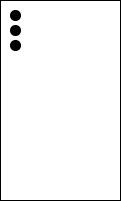
\includegraphics[scale=0.5]{img/rechenberg_notation/individuum.png}
	\caption{Individuum}
\label{fig:individuum}
\end{figure}
%population
\begin{figure}[!htb]
	\centering
	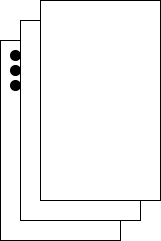
\includegraphics[scale=0.5]{img/rechenberg_notation/population.png}
	\caption{Population}
\label{fig:population}
\end{figure}
%population isoliert
\begin{figure}[!htb]
	\centering
	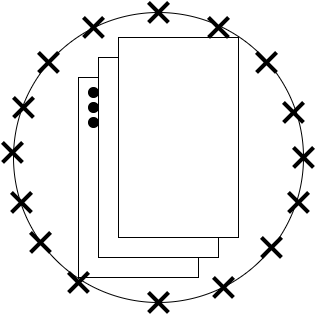
\includegraphics[scale=0.5]{img/rechenberg_notation/population_isoliert.png}
	\caption{Isolierte Population}
\label{fig:population_isoliert}
\end{figure}
%auswahl
\begin{figure}[!htb]
	\centering
	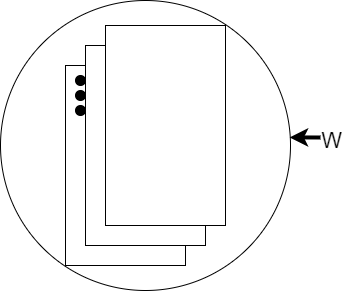
\includegraphics[scale=0.5]{img/rechenberg_notation/auswahl_gleichverteilt.png}
	\caption{Gleichverteilte Auswahl}
\label{fig:auswahl_gleichverteilt}
\end{figure}
\begin{figure}[!htb]
	\centering
	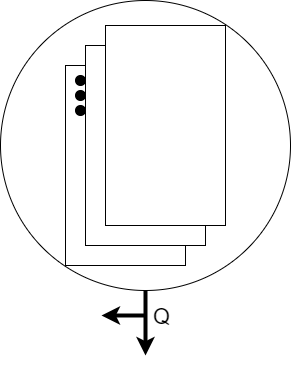
\includegraphics[scale=0.5]{img/rechenberg_notation/auswahl_qualitaetsfunktion.png}
	\caption{Auswahl mit einer Qualitätsfunktion}
\label{fig:auswahl_qualitaetsfunktion}
\end{figure}
%duplikation
\begin{figure}[!htb]
	\centering
	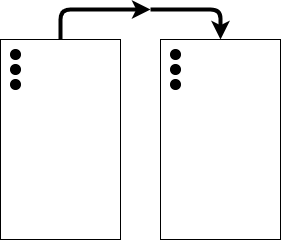
\includegraphics[scale=0.5]{img/rechenberg_notation/duplikation.png}
	\caption{Duplikation}
\label{fig:duplikation}
\end{figure}
%mutation
\begin{figure}[!htb]
	\centering
	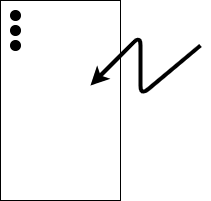
\includegraphics[scale=0.5]{img/rechenberg_notation/mutation.png}
	\caption{Mutation}
\label{fig:mutation}
\end{figure}
%bewertung
\begin{figure}[!htb]
	\centering
	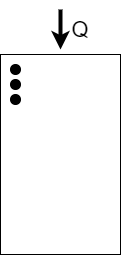
\includegraphics[scale=0.5]{img/rechenberg_notation/bewertung.png}
	\caption{Bewertung}
\label{fig:bewertung}
\end{figure}
%rekombination
\begin{figure}[!htb]
	\centering
	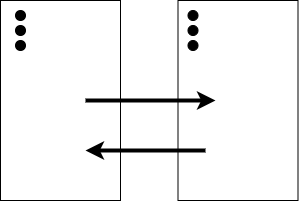
\includegraphics[scale=0.5]{img/rechenberg_notation/rekombination.png}
	\caption{Rekombination}
\label{fig:rekombination}
\end{figure}
%phänotypische realisierung
\begin{figure}[!htb]
	\centering
	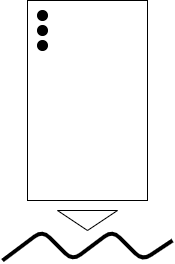
\includegraphics[scale=0.5]{img/rechenberg_notation/phaenotypische_realisation.png}
	\caption{Phänotypische Realisation}
\label{fig:phaenotypische_realisation}
\end{figure}


% 3. Typische Reihenfolge der Abschnitte kurz zeigen. Aber auch klar machen das das ganze extrem variieren kann
